% !TeX encoding = UTF-8
% !TeX program = pdflatex
% !TeX spellcheck = it_IT

\documentclass[a4paper,oneside,italian]{sapthesis}

% Pacchetti non già caricati da sapthesis
\usepackage[utf8]{inputenc}
\usepackage{microtype}
\usepackage{amssymb}
\usepackage{float}
\usepackage{array}
\usepackage{tabularx}
\usepackage{listings}
\usepackage{xcolor}
\usepackage{hyperref}
\usepackage{algorithm}
\usepackage{algpseudocode}

\hypersetup{
    colorlinks=true,
    linkcolor=black,
    citecolor=black,
    urlcolor=blue,
    pdftitle={Algoritmi per energy trading},
    pdfauthor={Daniele Quattrociocchi}
}

\setlength{\emergencystretch}{3em}

% ---------------------------------------------------------
% INFORMAZIONI TESI
% ---------------------------------------------------------

\title{Algoritmi per energy trading}
\author{Daniele Quattrociocchi}
\IDnumber{2024239}
\course{Laurea in Informatica}
\courseorganizer{Facoltà di Ingegneria dell'Informazione, Informatica e Statistica}
\AcademicYear{2025/2026}
\advisor{Prof.~Enrico Tronci}
\authoremail{quattrociocchi.2024239@studenti.uniroma1.it}
\copyyear{2026}
\thesistype{Relazione di Tirocinio}

% ---------------------------------------------------------
% CODICE
% ---------------------------------------------------------

\lstset{
    basicstyle=\ttfamily\small,
    breaklines=true,
    frame=single,
    numbers=left,
    numberstyle=\tiny,
    showstringspaces=false
}

\begin{document}

\frontmatter
\maketitle

\begin{abstract}
La relazione presenta un simulatore in C++ per confrontare strategie di compravendita
di energia elettrica su serie storiche di prezzi. Sono state analizzate una strategia
casuale e una basata sulla media geometrica dei prezzi, variando finestra storica,
soglia di acquisto e capitale accantonato. Nel dataset esaminato, la strategia basata
sulla media geometrica ha ottenuto rendimenti medi dal 4.57\% al 12.25\%, rispetto
allo 0.60\%--1.32\% della strategia casuale, con una variabilità maggiore nelle
configurazioni più redditizie.
\end{abstract}

\tableofcontents

\mainmatter

% =========================================================
% 1. INTRODUCTION
% =========================================================

\chapter{Introduzione}


\section{Contesto}

Il progetto si inserisce all'interno della materia di gestione
della compravendita di energia.
Per questo motivo è stato creato un simulatore in C++ in grado
di effettuare un confronto tra diverse strategie.
L'obiettivo del lavoro è studiare l'efficienza di una determinata
strategia "intelligente", ponendo come base una strategia che utilizza
scelte casuali. Le simulazioni sono state effettuate sui dati forniti,
che permettono di raccogliere e studiare i risultati delle due strategie,
per metterli in seguito a confronto.



\section{Motivazioni}

La motivazione principale che ha spinto la creazione di questo progetto 
è stata cercare di capire se un determinato algoritmo di decisione, diverso
dalla scelta casuale, fosse effettivamente più efficiente.
Inoltre, volevo realizzare in modo efficiente un simulatore in C++,
in grado di studiare il comportamento di diverse strategie utilizzando dati storici.

\clearpage
\section{Contributi}

I principali contributi del lavoro sono:

\begin{itemize}

    \item la progettazione e l'implementazione di un simulatore in C++
          per permettere lo svolgimento di test basati su algoritmi di compravendita;

    \item la modellazione dei principali elementi del dominio, tra cui
          batteria, portafoglio, transazioni e rete elettrica;

    \item l'implementazione e il confronto di strategie casuali e basate sulla
          media geometrica dei prezzi storici;

    \item la definizione di una campagna sperimentale per analizzare il
          rendimento medio e la sua variabilità al variare dei parametri.

\end{itemize}

% =========================================================
% 2. BACKGROUND
% =========================================================

\chapter{Contesto}
\label{chap:background}

Per rendere il progetto più semplice da comprendere e da modificare in seguito, 
è stato diviso in più moduli. Questa suddivisione permette di mantenere separate 
le diverse responsabilità degli elementi che compongono il progetto e di facilitare 
l'individuazione dei problemi nel momento in cui si presentano.

In particolare, i suoi moduli sono i seguenti.

\section{Batteria}

La batteria è il modulo che si occupa di mantenere i dati riguardanti la carica 
e la disponibilità di spazio rimanente al suo interno.

In particolare, attraverso la batteria possiamo immagazzinare energia e rimuoverla 
nel momento della vendita. Sono inoltre presenti dei controlli che impediscono 
il caricamento oltre la capacità massima e lo scaricamento oltre la quantità 
di energia disponibile.

\begin{figure}[ht]
    \centering
    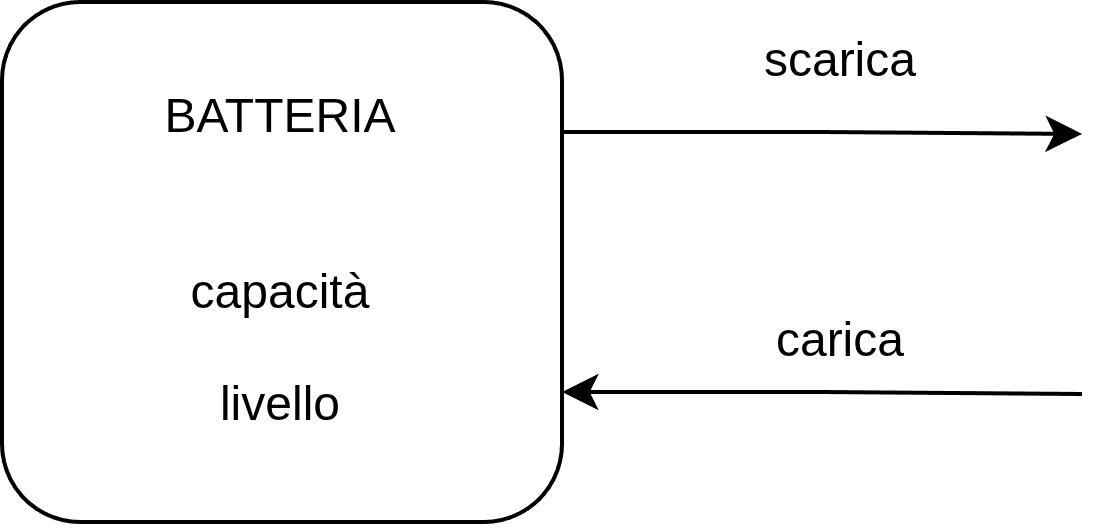
\includegraphics[width=0.5\textwidth]{../immagini/Batteria.png}
    \caption{Rappresentazione della batteria.}
    \label{fig:batteria}
\end{figure}

\clearpage

\section{Rete elettrica}

La rete elettrica è il modulo che permette di gestire lo storico dei prezzi e definire, per ogni rete, i relativi timestamp e prezzi.

Il modulo definisce il modello utilizzato per rappresentare ogni rete elettrica, 
ognuna delle quali possiede la propria sequenza di prezzi associata ai diversi 
timestamp.


\begin{figure}[ht]
    \centering
    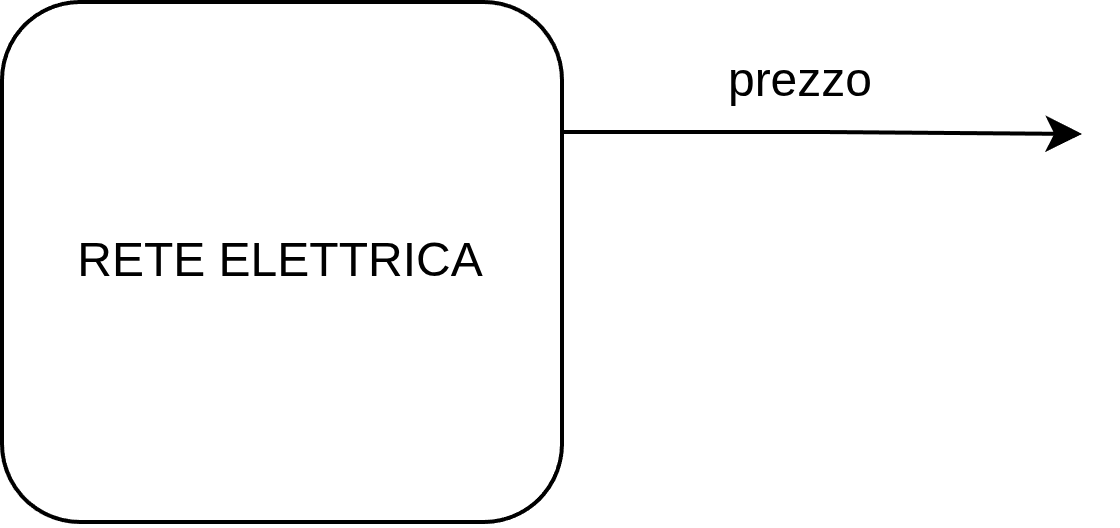
\includegraphics[width=0.5\textwidth]{../immagini/Rete_Elettrica.png}
    \caption{Rappresentazione della rete elettrica.}
    \label{fig:rete_elettrica}
\end{figure}

\section{Portafoglio}

Il portafoglio è un modulo essenziale che garantisce la gestione del denaro 
durante la simulazione.

Il suo saldo viene suddiviso in due parti, definite attraverso i parametri 
\texttt{SET\_ASIDE} e \texttt{AVAILABLE}. Possiamo quindi definire inizialmente 
una parte del saldo che non verrà utilizzata per nuovi acquisti e un'altra parte 
che potrà invece essere utilizzata per effettuare nuove operazioni.

Anche se solo una parte del saldo è disponibile per essere spesa, la somma 
delle due componenti costituisce il totale di cui dispone il portafoglio.


\begin{figure}[ht]
    \centering
    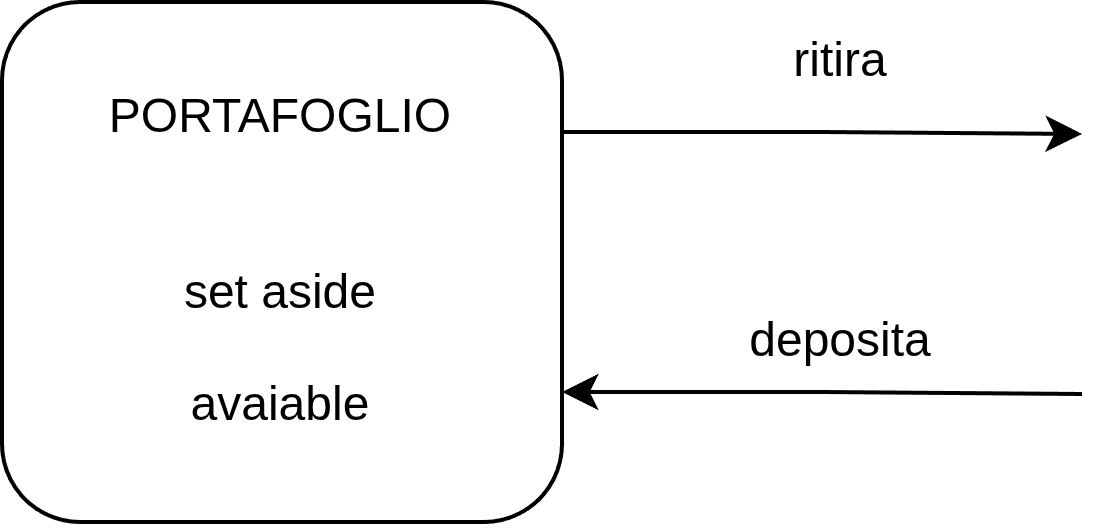
\includegraphics[width=0.5\textwidth]{../immagini/Portafoglio.png}
    \caption{Rappresentazione del portafoglio.}
    \label{fig:portafoglio}
\end{figure}

\section{Transazione}

Al fine di definire in maniera più precisa l'acquisto e la vendita di energia, 
è stato definito un modulo che riguarda nello specifico ogni transazione effettuata.

Grazie ad esso è possibile memorizzare le informazioni relative a una transazione, 
tra cui la quantità di energia acquistata o venduta e il relativo costo.

\section{Servizio di trading}

Questo particolare modulo permette di definire se è possibile effettuare 
un acquisto o una vendita.

In particolare, espone delle funzioni che permettono di verificare se è possibile 
effettuare una determinata operazione, considerando i vincoli relativi al 
portafoglio e alla batteria.

Inoltre, il modulo si occupa di eseguire le operazioni di acquisto e vendita 
una volta verificato che le condizioni necessarie siano rispettate.


\begin{figure}[ht]
    \centering
    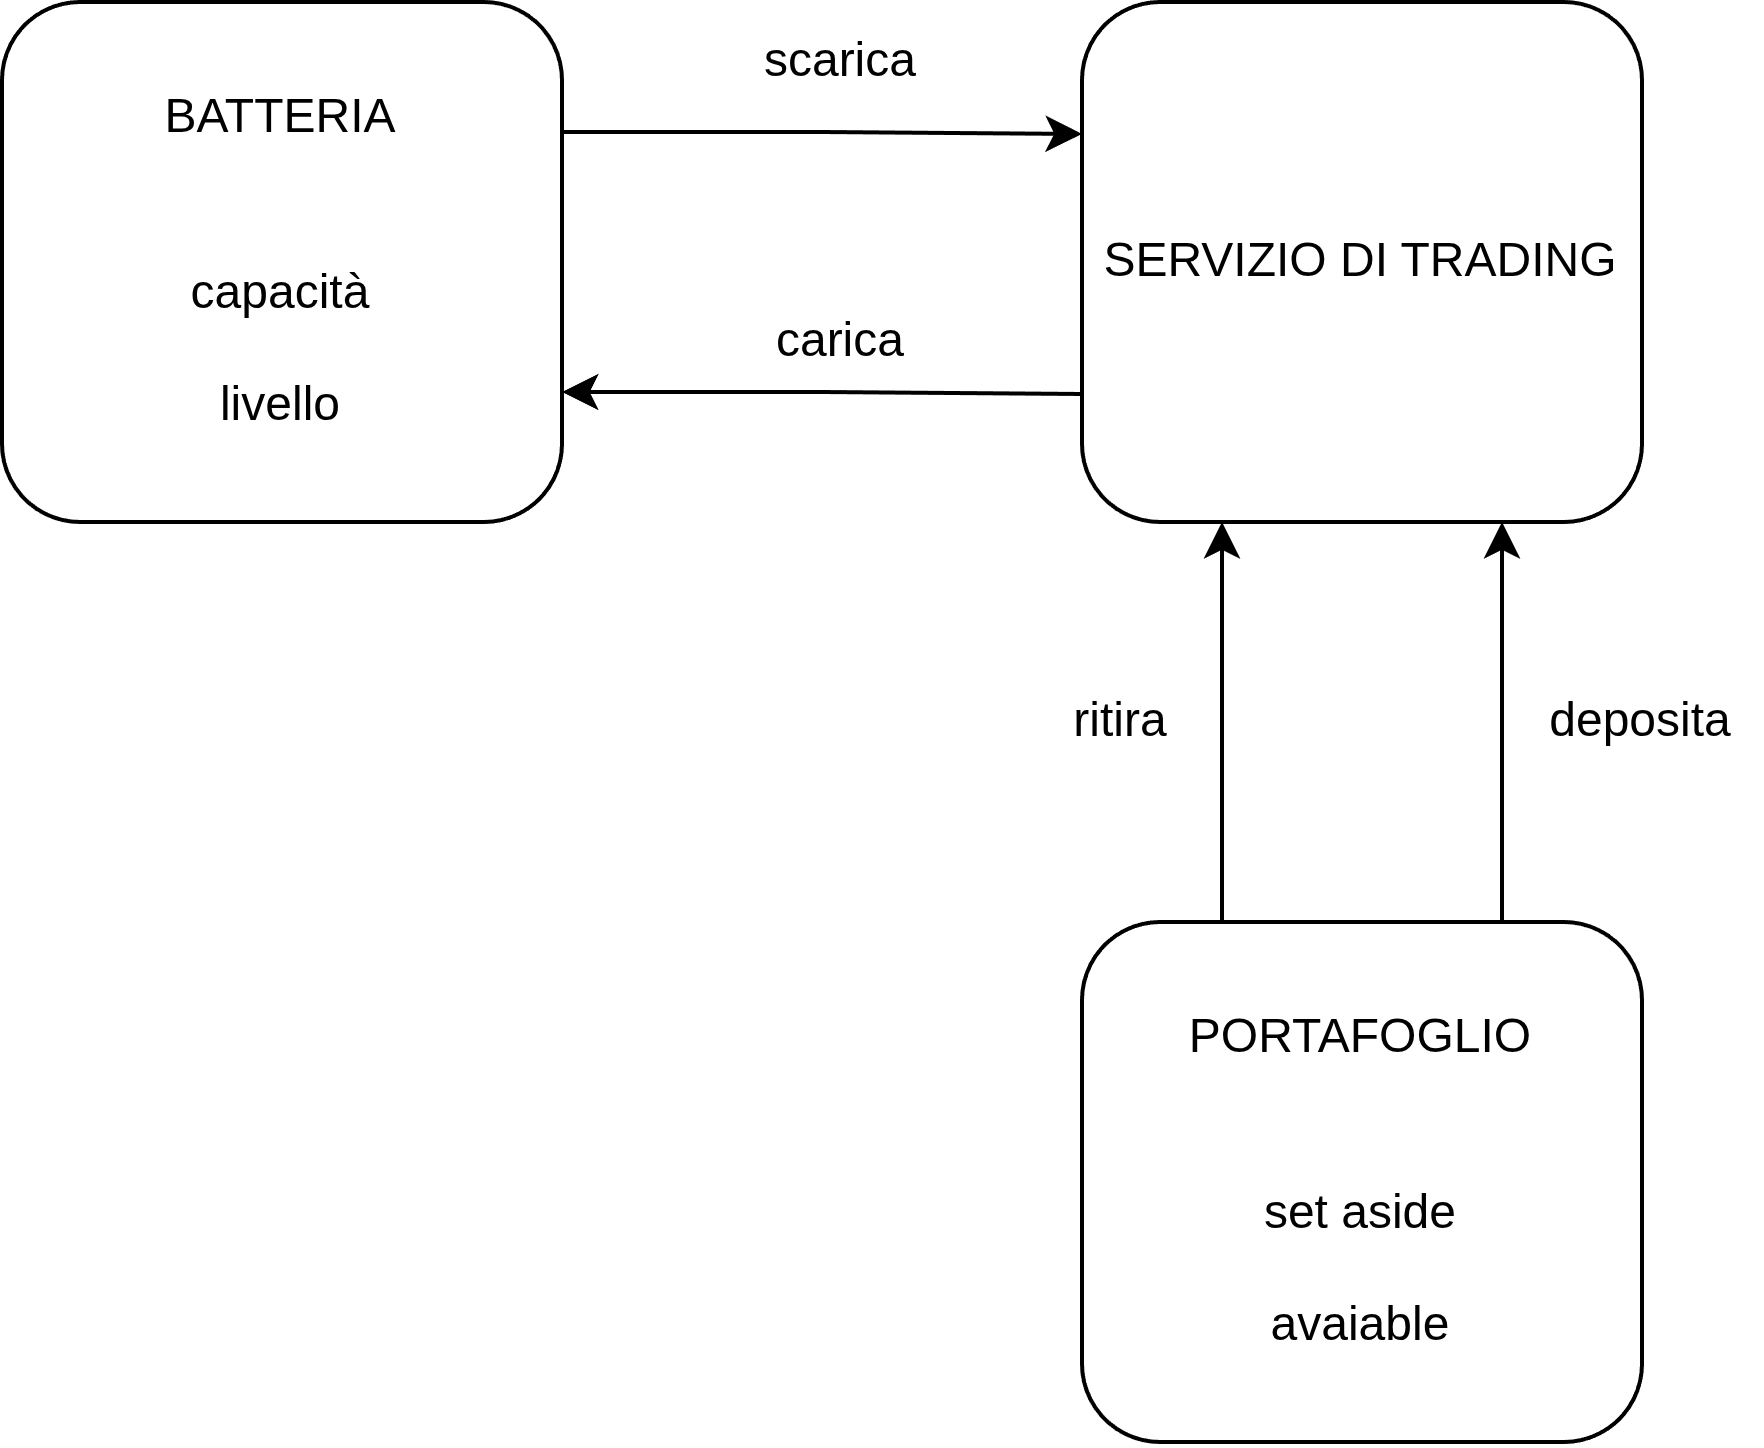
\includegraphics[width=0.5\textwidth]{../immagini/Servizio_Di_Trading.png}
    \caption{Rappresentazione del servizio di trading.}
    \label{fig:servizio di trading}
\end{figure}

\clearpage

\section{Strategie}

Per semplicità, sono state raccolte nello stesso modulo le due strategie 
utilizzate nel progetto. È inoltre possibile aggiungere facilmente altre 
strategie nel momento in cui si voglia effettuare un nuovo tipo di scelta.

Più nello specifico, una strategia corrisponde ad una funzione in grado di 
ricevere come parametri la batteria, l'array di reti elettriche, il portafoglio 
e il trading service.

\begin{itemize}
    \item \texttt{randomChoise}: a ogni timestamp seleziona casualmente, 
    con probabilità uniforme, una delle azioni disponibili: non operare, 
    acquistare o vendere. Le operazioni vengono comunque eseguite solo 
    quando il portafoglio e la batteria rispettano i vincoli necessari;

    \item \texttt{smartgeometricChoise}: ordina le reti in base al rapporto 
    prezzo/media geometrica, privilegiando gli acquisti sulle reti con 
    rapporto più basso e le vendite su quelle con rapporto più alto, 
    nel rispetto dei limiti massimi di acquisto e vendita.
\end{itemize}


\begin{figure}[ht]
    \centering
    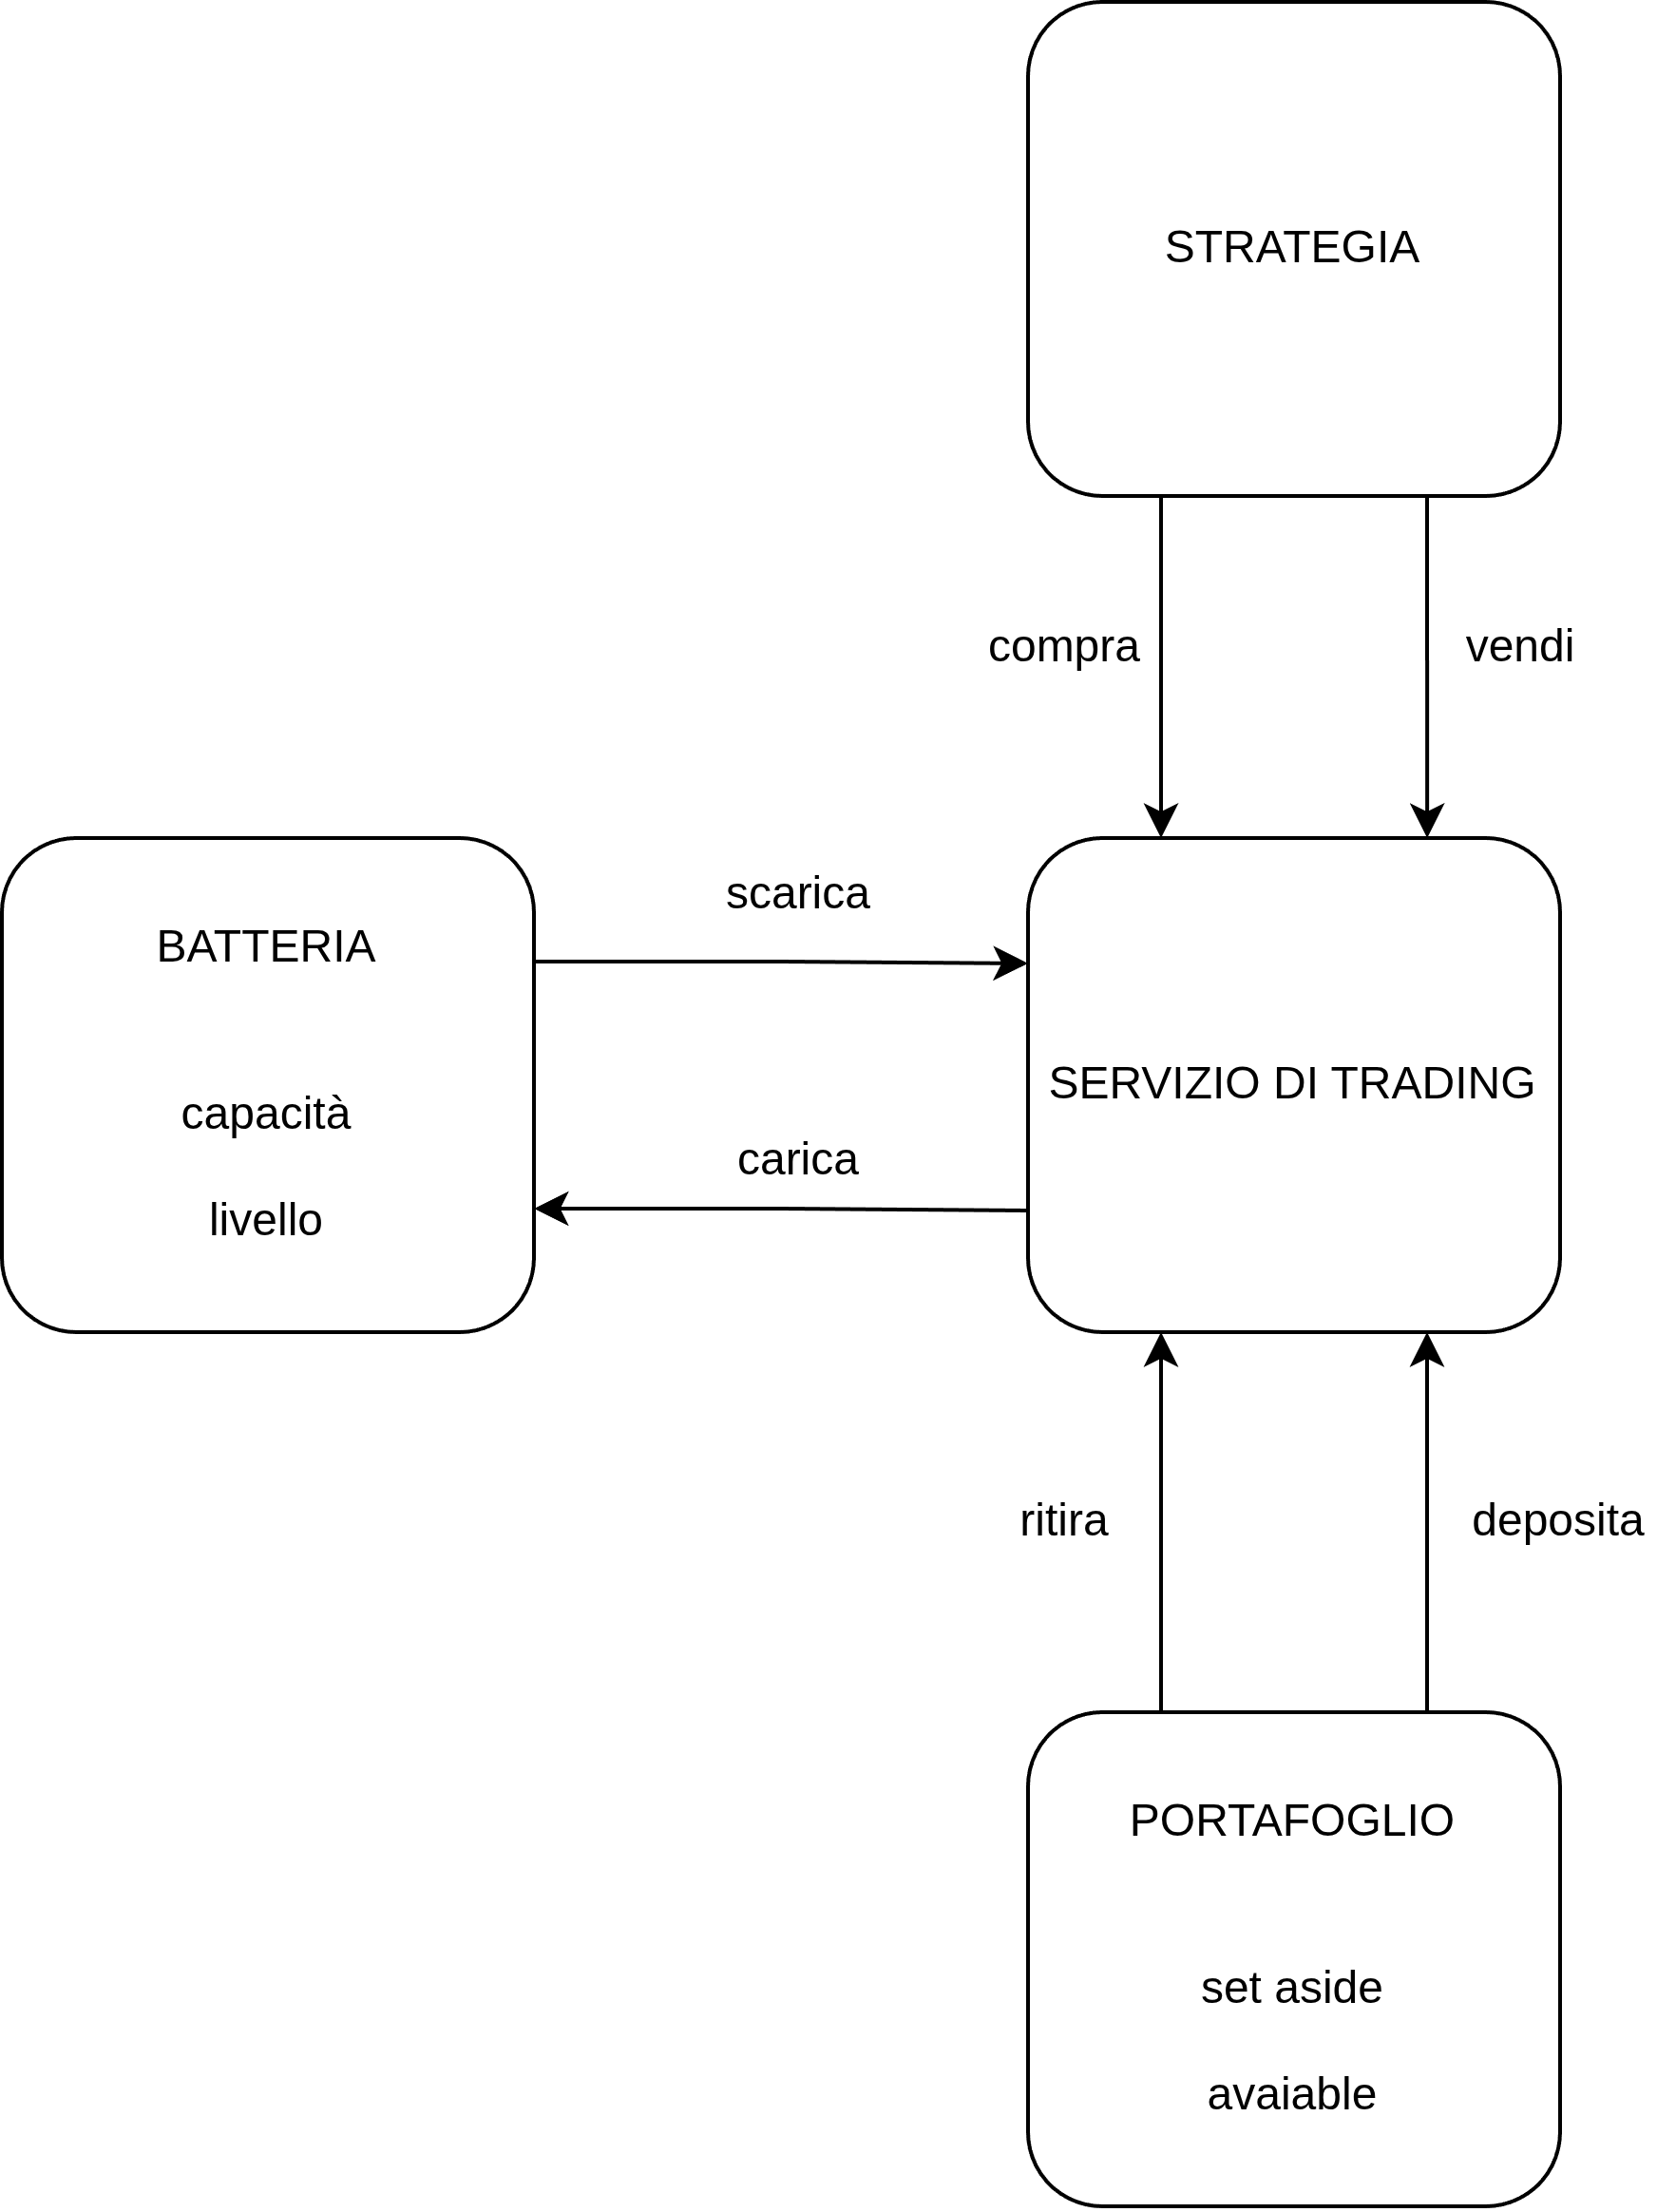
\includegraphics[width=0.5\textwidth]{../immagini/Strategia.png}
    \caption{Rappresentazione della strategia.}
    \label{fig:strategia}
\end{figure}

% =========================================================
% 3. METODOLOGIA
% =========================================================

\chapter{Metodologia}

\label{chap:methods}


% =========================================================
% 3.1 DEFINIZIONE DEL PROBLEMA
% =========================================================

\section{Definizione del problema}

Il problema affrontato consiste nel valutare se una strategia basata sui
prezzi storici possa ottenere risultati migliori rispetto a una strategia
casuale nella compravendita di energia elettrica.

L'obiettivo è quindi confrontare una strategia che non utilizza informazioni
relative all'andamento dei prezzi con una strategia che utilizza lo storico
dei prezzi per effettuare le proprie decisioni.


% =========================================================
% 3.2 APPROCCIO PROPOSTO
% =========================================================

\section{Approccio proposto}

Per valutare l'efficacia di una strategia è necessario disporre di un
riferimento con cui confrontare i risultati ottenuti. Per questo motivo è
stata inizialmente elaborata una strategia casuale, utilizzata come baseline.

La strategia random sceglie casualmente quale operazione effettuare, senza
utilizzare informazioni relative all'andamento dei prezzi. Essendo legata al
caso, rappresenta una strategia che non tiene conto della possibilità che
l'operazione scelta possa portare a un profitto. Essa viene quindi utilizzata
come riferimento per valutare se una strategia basata sulle informazioni
disponibili sui prezzi sia in grado di ottenere risultati differenti.

Nello scegliere se acquistare o meno un determinato quantitativo di energia,
una delle poche informazioni disponibili è lo storico dei prezzi. Grazie ad
esso è possibile analizzare il comportamento dei prezzi osservato in un
determinato intervallo temporale e individuare un valore di riferimento per
le decisioni di acquisto e vendita.

Una prima possibilità consiste nell'utilizzare una semplice media dei prezzi
osservati. Tuttavia, la media aritmetica considera i valori sulla base delle
loro differenze assolute. Nel caso dei prezzi, può invece essere interessante
considerare anche la loro variazione relativa. Ad esempio, un aumento da
50 a 100 e un aumento da 100 a 200 rappresentano in entrambi i casi un
raddoppio del prezzo, nonostante la differenza assoluta sia diversa.

Per questo motivo, nella strategia proposta viene utilizzata la media
geometrica dei prezzi osservati nella finestra temporale considerata. Essa
permette di ottenere un valore di riferimento basato sulla relazione
moltiplicativa tra i prezzi, risultando coerente con l'obiettivo di considerare
le variazioni relative anziché esclusivamente quelle assolute.


% =========================================================
% 3.3 PROGETTAZIONE DEL SISTEMA
% =========================================================

\section{Progettazione del sistema}

Il sistema è stato progettato per permettere l'esecuzione di numerosi
esperimenti mantenendo indipendenti i diversi scenari simulati. Ogni
esperimento viene gestito principalmente dal simulatore, che rappresenta
il cuore del progetto.

Nel momento in cui viene avviato il simulatore, vengono eseguite una serie
di operazioni necessarie per preparare l'esperimento. Come prima cosa viene
istanziato il database, che permette di gestire in modo più ordinato i dati
provenienti dai file CSV. Successivamente, i dati vengono caricati all'interno
del programma per poter essere utilizzati durante gli esperimenti.

Ogni esperimento utilizza i dati caricati per eseguire le operazioni previste
dalla strategia scelta e calcolare i relativi risultati. Per migliorare i tempi
di esecuzione, gli esperimenti vengono eseguiti in parallelo utilizzando i
core disponibili.

Ogni esperimento utilizza indipendentemente dagli altri una propria batteria
e un proprio portafoglio, in modo da evitare che lo stato di un esperimento
possa influenzare i risultati degli altri.


% =========================================================
% 3.4 METRICHE DI VALUTAZIONE
% =========================================================

\section{Metriche di valutazione}

Nel progetto vengono utilizzate alcune metriche di valutazione per analizzare
i risultati degli esperimenti e mettere in evidenza le differenze tra le
strategie considerate.

Di seguito vengono descritti i calcoli utilizzati.


\subsection{Yield}

Per calcolare il rendimento di una strategia viene utilizzato lo Yield,
definito come:

\begin{equation}
    Y = \frac{B_f - B_0}{B_0},
\end{equation}

dove $B_0$ è il saldo iniziale e $B_f$ è il saldo totale al termine della
finestra di simulazione, ottenuto sommando il saldo disponibile e quello
accantonato.

Al termine degli esperimenti viene calcolata la media degli Yield ottenuti,
considerando tutti i valori calcolati con i parametri impostati inizialmente.
Questo permette di ottenere un valore medio di riferimento per gli esperimenti
eseguiti con una determinata configurazione dei parametri.


\subsection{Deviazione standard}

Per valutare non solo il rendimento medio della strategia, ma anche la
variabilità dei risultati ottenuti nelle diverse simulazioni, viene calcolata
la deviazione standard dei rendimenti. Un valore elevato indica una maggiore
dispersione dei rendimenti rispetto al loro valore medio, mentre un valore più
basso indica risultati più concentrati attorno alla media.

Nel simulatore viene utilizzata la deviazione standard campionaria, calcolata
sui rendimenti prodotti dalle simulazioni. La formula utilizzata è:

\begin{equation}
\sigma =
\sqrt{
\frac{1}{n-1}
\sum_{i=1}^{n}
\left(y_i-\bar{y}\right)^2
}
\end{equation}

dove $y_i$ rappresenta il rendimento ottenuto dalla $i$-esima simulazione,
$\bar{y}$ rappresenta il rendimento medio e $n$ il numero complessivo di
simulazioni.

La deviazione standard $\sigma$ permette quindi di affiancare al rendimento
medio una misura della dispersione dei risultati, fornendo un'indicazione
della variabilità associata alla strategia.


% =========================================================
% 3.5 ALGORITMI
% =========================================================

\section{Algoritmi}

Nel progetto sono stati sviluppati due algoritmi differenti per effettuare
le decisioni di acquisto e vendita. Di seguito vengono descritte le due
strategie utilizzate per effettuare il confronto tra i loro risultati.


% =========================================================
% 3.5.1 ALGORITMO RANDOM
% =========================================================

\subsection{Algoritmo random}

L'algoritmo random effettua una scelta casuale per ogni timestamp e per ogni
rete elettrica tra le possibili operazioni. In particolare, vengono
considerate tre possibilità: non effettuare alcuna operazione, acquistare
energia oppure vendere energia.

La scelta viene effettuata utilizzando una distribuzione uniforme discreta.
Le tre operazioni hanno quindi la stessa probabilità di essere selezionate:

\begin{equation}
P(\text{nessuna operazione}) =
P(\text{acquisto}) =
P(\text{vendita}) =
\frac{1}{3}.
\end{equation}

La scelta casuale viene effettuata utilizzando un generatore di numeri
pseudo-casuali inizializzato mediante una sorgente di casualità fornita
dal sistema.

L'operazione scelta non viene però eseguita direttamente. Prima di effettuare
l'operazione vengono verificati i vincoli necessari attraverso il servizio
di trading. Ad esempio, non è possibile acquistare energia se il portafoglio
non dispone del denaro necessario, così come non è possibile vendere energia
se la batteria non contiene una quantità sufficiente di energia.

Se i vincoli necessari sono rispettati, viene eseguita l'operazione
selezionata. In caso contrario, l'operazione non viene effettuata.

In questo modo la strategia random non utilizza informazioni relative ai
prezzi storici per determinare l'azione da intraprendere e costituisce la
baseline utilizzata per confrontare i risultati ottenuti dalla strategia
\texttt{smartgeometricChoise}.


% =========================================================
% 3.5.2 ALGORITMO SMART
% =========================================================

\subsection{Algoritmo \texttt{smartgeometricChoise}}

La strategia \texttt{smartgeometricChoise} utilizza lo storico dei prezzi
per determinare quali operazioni effettuare. In particolare, per ogni rete
elettrica viene calcolata la media geometrica dei prezzi presenti nella
finestra storica considerata.

La media geometrica utilizzata dalla strategia è calcolata come:

\begin{equation}
    G =
    \exp\left(
        \frac{1}{n}
        \sum_{k=1}^{n}
        \log p_k
    \right),
\end{equation}

dove $p_k$ sono i prezzi validi nella finestra storica e $n$ è il loro numero.

Indicando con $p$ il prezzo corrente, la decisione viene effettuata
attraverso il rapporto tra il prezzo corrente e la media geometrica:

\begin{equation}
    r = \frac{p}{G}.
\end{equation}

Un valore del rapporto inferiore a $1$ indica che il prezzo corrente è
inferiore alla media geometrica, mentre un valore superiore a $1$ indica
che il prezzo corrente è superiore alla media.

La strategia utilizza quindi due soglie per determinare le operazioni.
Si acquista quando il rapporto $r$ è inferiore alla soglia di acquisto,
mentre si vende quando il rapporto $r$ è superiore alla soglia di vendita.

Le reti elettriche vengono ordinate in base al rapporto calcolato. Gli acquisti
vengono effettuati partendo dalle reti con il rapporto più basso, mentre le
vendite vengono effettuate partendo da quelle con il rapporto più alto.

Le operazioni sono comunque soggette ai limiti massimi di acquisto e vendita
e ai vincoli del portafoglio e della batteria.
% =========================================================
% 4. IMPLEMENTATION
% =========================================================

\chapter{Implementazione}

\label{chap:implementation}

\section{Architettura del sistema}

Per una questione di velocità nella lettura ed elaborazione dei dati si è decidso
di creare il progetto nel linguaggio c++, il progetto è suddiviso in classi che 
ne rendono la comprensione e l'organizzazione molto più semplice.
Nello sviluppare il tutto infatti ogni componente è stata racchiusa all'interno di 
una classe, infatti possiamo definirli attraverso metodi e attributi che ne indicano 
lo stato e le azioni.
Di seguito viene spiegato in pseudocodice come ogni componente è stato sviluppato 
partendo appunto dalle classi più importanti che ne determinano il funzionamento 

\subsection{Batteria}

Per l'implementazione della batteria è stato necessario definire gli attributi
che ne rappresentano lo stato, in particolare il livello di energia
immagazzinata e la capacità massima dell'accumulatore. Sono stati inoltre
implementati i metodi necessari per effettuare le operazioni di carica e
scarica della batteria.

Prima di modificare il livello energetico viene verificato che l'operazione
richiesta sia compatibile con lo stato corrente della batteria. Di seguito
sono riportati gli pseudocodici relativi ai due metodi.

\begin{algorithm}[H]
\caption{Caricamento della batteria}
\label{alg:battery-charge}
\begin{algorithmic}[1]
\Require Quantità di energia $q$
\If{$q > capacity - level$}
    \State Genera un'eccezione
\Else
    \State $level \gets level + q$
\EndIf
\State \Return $q$
\end{algorithmic}
\end{algorithm}

\begin{algorithm}[H]
\caption{Scaricamento della batteria}
\label{alg:battery-discharge}
\begin{algorithmic}[1]
\Require Quantità di energia $q$
\If{$q > level$}
    \State Genera un'eccezione
\Else
    \State $level \gets level - q$
\EndIf
\State \Return $q$
\end{algorithmic}
\end{algorithm}

\subsection{Rete elettrica}

La classe \texttt{ElectricityGrid} rappresenta una rete elettrica e deriva
dalla classe \texttt{Source}. La classe mantiene lo storico dei prezzi
associati alla rete e fornisce i metodi necessari per aggiungere e recuperare
i prezzi corrispondenti ai diversi timestamp. Viene inoltre mantenuto
l'identificativo della sorgente, associato alla rete nel database.

Per rendere più efficiente il calcolo della media geometrica, la classe
mantiene inoltre due strutture ausiliarie. La prima contiene le somme
cumulative dei logaritmi dei prezzi, mentre la seconda mantiene il numero
cumulativo dei prezzi validi. Queste strutture permettono di ottenere le
informazioni relative a una finestra temporale senza dover analizzare
nuovamente tutti i prezzi contenuti nella finestra.

L'aggiornamento delle strutture cumulative viene effettuato quando viene
aggiunto un nuovo prezzo. Il seguente pseudocodice descrive tale operazione.

\begin{algorithm}[H]
\caption{Aggiornamento delle strutture cumulative}
\label{alg:electricity-grid-prefix}
\begin{algorithmic}[1]

\Require Valore logaritmico del prezzo

\If{la lista delle somme logaritmiche è vuota}
    \State Imposta la somma precedente a zero
\Else
    \State Recupera l'ultima somma logaritmica
\EndIf

\State Aggiungi la nuova somma alla lista delle somme logaritmiche

\If{l'ultimo prezzo inserito è maggiore di zero}
    \State Imposta il valore di validità a uno
\Else
    \State Imposta il valore di validità a zero
\EndIf

\If{la lista dei conteggi validi è vuota}
    \State Imposta il conteggio precedente a zero
\Else
    \State Recupera l'ultimo conteggio dei prezzi validi
\EndIf

\State Aggiorna il conteggio cumulativo dei prezzi validi

\end{algorithmic}
\end{algorithm}

Una volta costruite le somme cumulative, è possibile ottenere la somma dei
logaritmi relativa a una specifica finestra temporale senza dover percorrere
nuovamente tutti gli elementi.

\begin{algorithm}[H]
\caption{Calcolo della somma dei logaritmi}
\label{alg:electricity-grid-log-sum}
\begin{algorithmic}[1]

\Require Indice iniziale
\Require Indice finale

\If{l'indice iniziale è maggiore o uguale all'indice finale}
    \State \Return zero
\EndIf

\If{l'indice iniziale è zero}
    \State La somma è uguale all'ultimo valore cumulativo della finestra
\Else
    \State La somma è ottenuta sottraendo il valore cumulativo precedente
\EndIf

\State \Return la somma calcolata

\end{algorithmic}
\end{algorithm}

Lo stesso principio viene utilizzato per determinare il numero di prezzi
validi presenti nella finestra temporale.

\begin{algorithm}[H]
\caption{Conteggio dei prezzi validi}
\label{alg:electricity-grid-valid-count}
\begin{algorithmic}[1]

\Require Indice iniziale
\Require Indice finale

\If{l'indice iniziale è maggiore o uguale all'indice finale}
    \State \Return zero
\EndIf

\If{l'indice iniziale è zero}
    \State Il conteggio è uguale all'ultimo valore cumulativo
\Else
    \State Il conteggio è ottenuto sottraendo il valore cumulativo precedente
\EndIf

\State \Return il conteggio calcolato

\end{algorithmic}
\end{algorithm}

L'utilizzo delle somme cumulative permette quindi di recuperare le
informazioni necessarie al calcolo della media geometrica in modo più
efficiente rispetto alla scansione completa della finestra temporale.

\subsection{Portafoglio}

La classe \texttt{Wallet} rappresenta il portafoglio utilizzato dal simulatore
per la gestione del denaro associato alle operazioni di acquisto e vendita
dell'energia. Il saldo del portafoglio è suddiviso in una parte disponibile
per le transazioni e in una parte messa da parte, che non può essere
utilizzata per gli acquisti.

Al momento della creazione, il saldo disponibile viene inizializzato con il
valore del saldo iniziale, mentre la parte messa da parte viene inizializzata
a zero. La classe mette inoltre a disposizione metodi per ottenere i due
saldi separatamente e il saldo complessivo del portafoglio.

La gestione del portafoglio avviene principalmente attraverso le operazioni
di deposito e prelievo. Nel caso di un deposito, una parte dell'importo viene
messa da parte in base alla percentuale definita dalla configurazione,
mentre la parte restante viene aggiunta al saldo disponibile.

\begin{algorithm}[H]
\caption{Deposito nel portafoglio}
\label{alg:wallet-deposit}
\begin{algorithmic}[1]

\Require Importo da depositare

\State Calcola la quota da mettere da parte
\State Aggiungi la quota al saldo messo da parte
\State Calcola la quota disponibile
\State Aggiungi la quota al saldo disponibile
\State \Return il saldo disponibile

\end{algorithmic}
\end{algorithm}

Il prelievo, invece, può essere effettuato solamente se l'importo richiesto
non supera il saldo disponibile. In caso contrario viene generata
un'eccezione; se il controllo ha esito positivo, l'importo viene sottratto
dal saldo disponibile.

\begin{algorithm}[H]
\caption{Prelievo dal portafoglio}
\label{alg:wallet-withdraw}
\begin{algorithmic}[1]

\Require Importo da prelevare

\If{l'importo supera il saldo disponibile}
    \State Genera un'eccezione
\Else
    \State Sottrai l'importo dal saldo disponibile
\EndIf

\State \Return il saldo disponibile

\end{algorithmic}
\end{algorithm}

\subsection{Transazione}

La struttura \texttt{Transaction} rappresenta una singola transazione
effettuata durante la simulazione. Essa contiene un riferimento alla
sorgente energetica coinvolta, la quantità di energia scambiata, il prezzo
dell'operazione e il saldo associato alla transazione.

La struttura contiene inoltre un valore booleano che permette di distinguere
le operazioni di vendita da quelle di acquisto. In particolare, il valore
\texttt{true} identifica una vendita, mentre il valore \texttt{false}
identifica un acquisto.

\subsection{Simulatore}

La classe \texttt{Simulator} rappresenta il componente responsabile
dell'esecuzione delle simulazioni. Essa riceve un riferimento al database
contenente i dati delle reti elettriche e il tipo di strategia da utilizzare.
Il simulatore coordina quindi l'interazione tra le reti elettriche, la
batteria, il portafoglio e il servizio di trading durante l'esecuzione
dell'esperimento.

Il metodo principale della classe è \texttt{run()}, che inizialmente carica
dal database le reti elettriche utilizzate dalla simulazione. Successivamente
vengono considerate le diverse finestre temporali definite dai parametri
dell'esperimento. Per ogni finestra vengono inizializzati una nuova batteria,
un nuovo portafoglio e una nuova istanza del servizio di trading.

All'interno di ogni finestra viene quindi eseguito un ciclo sui timestamp
considerati. A ogni iterazione viene selezionata la strategia configurata
per il simulatore e viene eseguita la relativa funzione. Al termine della
finestra, le eventuali posizioni ancora presenti vengono liquidate e il
rendimento ottenuto viene aggiunto all'insieme dei risultati dell'esperimento.

Il funzionamento complessivo del metodo \texttt{run()} può essere
rappresentato dal seguente pseudocodice.

\begin{algorithm}[H]
\caption{Esecuzione della simulazione}
\label{alg:simulator-run}
\begin{algorithmic}[1]

\State Carica le reti elettriche dal database

\For{ogni finestra temporale}
    \State Inizializza la batteria
    \State Inizializza il portafoglio
    \State Inizializza il servizio di trading

    \For{ogni timestamp della finestra}
        \State Seleziona la strategia configurata
        \State Esegui la strategia selezionata
    \EndFor

    \State Liquida le posizioni rimanenti
    \State Calcola il rendimento della finestra
    \State Aggiungi il rendimento ai risultati
\EndFor

\State Calcola il rendimento medio
\State Calcola la deviazione standard
\State Registra i risultati dell'esperimento

\end{algorithmic}
\end{algorithm}

Una parte importante dell'implementazione riguarda la parallelizzazione
dell'esecuzione delle finestre temporali. Il ciclo esterno viene infatti
parallelizzato mediante OpenMP, mentre ogni finestra mantiene una propria
batteria, un proprio portafoglio e una propria istanza del servizio di
trading. Le finestre possono quindi essere elaborate indipendentemente,
riducendo il tempo complessivo necessario per l'esecuzione della campagna
di simulazione.

Al termine dell'elaborazione di tutte le finestre, il simulatore calcola il
rendimento medio e la deviazione standard dei risultati raccolti. I valori
ottenuti, insieme ai parametri dell'esperimento, vengono infine registrati
per le successive analisi.
% ======================================================================

\subsection{Gestione del database}

Il simulatore utilizza un database SQLite per la memorizzazione dei dati
relativi ai prezzi dell'energia. L'utilizzo di un database permette di
mantenere separati i dati utilizzati dagli esperimenti dalla logica del
simulatore e di recuperarli successivamente senza doverli rielaborare ad
ogni esecuzione.

Durante l'avvio della simulazione, i dati presenti nel database vengono
caricati in memoria e utilizzati per costruire gli oggetti
\texttt{ElectricityGrid}. In questo modo le operazioni effettuate durante
la simulazione non richiedono accessi continui al database, ma lavorano
direttamente sulle strutture presenti in memoria.

Questa scelta è particolarmente importante considerando la quantità di dati
utilizzata negli esperimenti. L'accesso al database viene quindi
concentrato nella fase iniziale dell'esecuzione, mentre le successive
operazioni di lettura dei prezzi vengono effettuate sulle strutture
ricostruite in memoria.

La separazione tra persistenza e simulazione permette inoltre di utilizzare
lo stesso insieme di dati per eseguire esperimenti differenti, modificando
solamente i parametri e la strategia utilizzata dal simulatore.

\section{Implementazione delle strategie}

Le strategie utilizzate dal simulatore sono implementate come funzioni che
ricevono le reti elettriche, il portafoglio, la batteria e il servizio di
trading. A ogni timestamp la strategia analizza le reti disponibili e
determina le eventuali operazioni di acquisto o vendita.

Nel progetto sono presenti due strategie: \texttt{Random},
\texttt{SmartGeometric}. Gli esperimenti descritti
nel seguito della tesi utilizzano la strategia casuale come
riferimento e la strategia \texttt{SmartGeometric} come strategia basata
sull'analisi dei prezzi storici.

\subsection{Strategia Random}

La strategia \texttt{Random} rappresenta una strategia di riferimento nella
quale la decisione relativa all'operazione da effettuare viene determinata
casualmente.

Per ogni rete elettrica viene innanzitutto recuperato il prezzo associato
al timestamp corrente. Se il prezzo non è disponibile, la rete viene
ignorata. In caso contrario viene generato casualmente un valore tra tre
possibili azioni: nessuna operazione, acquisto oppure vendita.

Nel caso di acquisto o vendita, l'operazione non viene eseguita
direttamente. Prima viene verificato attraverso il \texttt{TradingService}
che la transazione sia compatibile con lo stato corrente del portafoglio e
della batteria. Solo se il controllo ha esito positivo viene eseguita
l'operazione corrispondente.

La generazione delle azioni casuali utilizza un generatore
\texttt{std::mt19937} associato al singolo thread, insieme a una
distribuzione uniforme sugli interi compresi tra zero e due. In questo modo
le tre possibili azioni vengono selezionate con la stessa probabilità.

Il funzionamento della strategia può essere rappresentato dal seguente
pseudocodice.

\begin{algorithm}[H]
\caption{Strategia Random}
\label{alg:random-strategy}
\begin{algorithmic}[1]

\For{ogni rete elettrica}
    \State Recupera il prezzo al timestamp corrente

    \If{il prezzo non è disponibile}
        \State Ignora la rete
    \Else
        \State Genera casualmente un'azione tra nessuna operazione,
        acquisto e vendita

        \If{l'azione è acquisto}
            \If{l'acquisto è consentito}
                \State Esegui l'acquisto
            \EndIf

        \ElsIf{l'azione è vendita}
            \If{la vendita è consentita}
                \State Esegui la vendita
            \EndIf
        \EndIf
    \EndIf
\EndFor

\end{algorithmic}
\end{algorithm}

\subsection{Strategia SmartGeometric}

La strategia \texttt{SmartGeometric} utilizza invece le informazioni
storiche sui prezzi per determinare le operazioni da effettuare. Per ogni
rete viene calcolata la media geometrica relativa alla finestra temporale
considerata e viene determinato il rapporto tra il prezzo corrente e tale
media.

Il rapporto viene utilizzato come indicatore della posizione relativa del
prezzo corrente rispetto al valore storico di riferimento. Le reti vengono
inserite in una struttura ordinata in base a questo rapporto, dalla rete
con il valore più basso a quella con il valore più alto.

La fase di acquisto considera le reti a partire da quelle con il rapporto
più basso. Vengono considerate solamente le reti per le quali il rapporto
è inferiore alla soglia di acquisto. Inoltre, il numero di acquisti viene
limitato dal parametro \texttt{MAX\_BUY}. Prima di effettuare ogni
operazione viene comunque verificato attraverso il \texttt{TradingService}
che l'acquisto sia possibile.

La fase di vendita procede in maniera analoga, ma considera le reti
partendo da quelle con il rapporto più alto. Una vendita viene considerata
solo quando il rapporto supera la soglia di vendita e il numero massimo di
vendite non è stato raggiunto. Anche in questo caso l'operazione viene
effettuata solamente se il \texttt{TradingService} ne consente l'esecuzione.

La strategia utilizza quindi sia le soglie definite nella configurazione
sia l'ordinamento delle reti, permettendo di dare priorità alle opportunità
di acquisto e vendita maggiormente distanti dalla relativa media
geometrica.

Il funzionamento complessivo della strategia è rappresentato nel seguente
pseudocodice.

\begin{algorithm}[H]
\caption{Strategia SmartGeometric}
\label{alg:smart-geometric-strategy}
\begin{algorithmic}[1]

\State Crea una struttura per memorizzare i rapporti
\State prezzo corrente / media geometrica

\For{ogni rete elettrica}
    \State Recupera il prezzo al timestamp corrente

    \If{il prezzo non è disponibile}
        \State Ignora la rete
    \Else
        \State Calcola la media geometrica della rete

        \If{la media geometrica non è valida}
            \State Ignora la rete
        \Else
            \State Calcola il rapporto tra prezzo corrente e media geometrica
            \State Inserisci il rapporto e la rete nella struttura ordinata
        \EndIf
    \EndIf
\EndFor

\State Inizializza il contatore degli acquisti

\For{le reti ordinate dal rapporto più basso}
    \If{il rapporto raggiunge la soglia di acquisto}
        \State Termina la fase di acquisto
    \EndIf

    \If{è stato raggiunto il numero massimo di acquisti}
        \State Termina la fase di acquisto
    \EndIf

    \If{l'acquisto è consentito}
        \State Esegui l'acquisto
    \EndIf
\EndFor

\State Inizializza il contatore delle vendite

\For{le reti ordinate dal rapporto più alto}
    \If{il rapporto raggiunge la soglia di vendita}
        \State Termina la fase di vendita
    \EndIf

    \If{è stato raggiunto il numero massimo di vendite}
        \State Termina la fase di vendita
    \EndIf

    \If{la vendita è consentita}
        \State Esegui la vendita
    \EndIf
\EndFor

\end{algorithmic}
\end{algorithm}

% =========================================================
% 5. VALUTAZIONE SPERIMENTALE
% =========================================================

\chapter{Valutazione sperimentale}
\label{chap:results}

% ---------------------------------------------------------
% CONFIGURAZIONE SPERIMENTALE
% ---------------------------------------------------------

\section{Configurazione sperimentale}

La campagna sperimentale è stata eseguita sul simulatore compilato in
ambiente locale. I prezzi sono stati caricati nel database SQLite a partire
dal file di dati e ogni configurazione è stata eseguita su finestre temporali
di 300 timestamp. Il confronto utilizza la stessa durata, lo stesso saldo
iniziale e lo stesso budget per operazione, variando soltanto i parametri
oggetto dell'analisi.

\subsection{Hardware}

Per gli esperimenti è stato utilizzato un computer locale con:
\begin{itemize}
    \item \texttt{disco}: nvme 970 evo plus;
    \item \texttt{ram}: 16 GB;
    \item \texttt{processore}: Intel Core i7-9700;
\end{itemize}

Sono riportate soltanto le caratteristiche considerate rilevanti per
l'esecuzione degli esperimenti.

\subsection{Software}

Il simulatore è sviluppato in C++ e utilizza le seguenti librerie e tecnologie esterne \cite{cppreference}:
\begin{itemize}
    \item \texttt{SQLite} per la gestione del database interno \cite{sqlite};
    \item \texttt{OpenMP} per la parallelizzazione delle simulazioni \cite{openmp}.
\end{itemize}

\subsection{Parametri}

I test sono stati eseguiti mantenendo fissi la durata della simulazione, il
budget per operazione, il saldo iniziale e la soglia di vendita. Sono stati
variati la finestra geometrica, la percentuale accantonata e la soglia di
acquisto, secondo i valori riportati in Tabella~\ref{tab:experimental-parameters}.



\begin{table}[H]
    \centering
    \caption{Parametri utilizzati nella campagna sperimentale.}
    \label{tab:experimental-parameters}
    \begin{tabular}{ll}
        \toprule
        Parametro & Valori considerati \\
        \midrule
        Finestra simulazione & 300 \\
        Budget per operazione & 10 \\
        Saldo iniziale & 1000 \\
        Set Aside (\%) & 10, 20, 30, 50 \\
        Finestra geometrica & 10, 20, 50, 100 \\
        Buy Threshold & 0.9, 0.8, 0.7 \\
        Sell Threshold & 1.0 \\
        \bottomrule
    \end{tabular}
\end{table}

La strategia \texttt{randomChoise} non utilizza la finestra geometrica né le
soglie di acquisto e vendita per prendere le decisioni: per ogni rete e per
ogni istante seleziona casualmente l'azione da eseguire. Per questo motivo non
è metodologicamente corretto associare una singola riga Smart a una riga
Random avente gli stessi valori di tutti i parametri. Random viene invece
trattata come baseline, mentre i parametri specifici della strategia Smart
sono analizzati separatamente.

% va bene 

% ---------------------------------------------------------
% CASI DI STUDIO
% ---------------------------------------------------------

\section{Casi di studio}

I casi di studio sono costruiti a partire dalle combinazioni dei parametri
riportati nella sezione precedente. Per ogni configurazione vengono raccolti
il rendimento medio (\textit{Average Yield}), la deviazione standard e la
variazione media del saldo finale.

\subsection{Baseline casuale}

La strategia \texttt{randomChoise} costituisce il riferimento sperimentale
utilizzato per il confronto con la strategia basata sui prezzi storici.

Nel campione analizzato produce un rendimento medio compreso tra 0.604743\%
e 1.31554\%, mentre la deviazione standard varia tra 4.38354\% e 8.57587\%.
La variazione media del saldo finale è compresa tra 6.04743 e 13.1554 unità monetarie.

Al variare della percentuale di capitale accantonato, il rendimento non segue
un andamento monotono: passa da 0.604743\% con il 10\% di capitale accantonato
a 1.28263\% con il 20\%, raggiunge 1.31554\% con il 30\% e scende a 1.09330\%
con il 50\%.

La deviazione standard diminuisce invece progressivamente, passando dall'8.57587\%
con il 10\% di capitale accantonato al 4.38354\% con il 50\%.

\subsection{Strategia Smart}

Per la strategia \texttt{smartgeometricChoise} sono state analizzate quattro
diverse finestre geometriche e tre diverse soglie di acquisto. Per ogni
combinazione sono state inoltre considerate le diverse percentuali di
capitale accantonato utilizzate negli esperimenti.

A differenza della strategia casuale, la strategia Smart utilizza quindi
parametri specifici legati al calcolo della media geometrica e alla scelta
delle operazioni da effettuare. I risultati ottenuti vengono confrontati con
la baseline casuale, osservando come il rendimento e la sua variabilità
cambiano al variare dei diversi parametri.

% va bene 

% ---------------------------------------------------------
% CORRETTEZZA
% ---------------------------------------------------------

\section{Correttezza}

La correttezza del sistema è stata valutata definendo all'interno del codice
una serie di controlli che impediscono di discostarsi dai vincoli previsti
dal modello. In particolare, sono state effettuate delle scelte di
progettazione come il controllo degli acquisti, che non possono essere
effettuati se non si possiede il denaro necessario, oppure il controllo delle
vendite, che possono essere effettuate solo se si possiede una quantità
sufficiente di energia elettrica.

Altri controlli riguardano la batteria, che non può contenere una quantità di
energia superiore alla capacità per cui è stata progettata.

Tutti questi controlli permettono di effettuare gli esperimenti mantenendo
il rispetto dei vincoli definiti dal sistema. In caso di errore o di
violazione di uno dei vincoli, vengono sollevate delle eccezioni che
interrompono l'esecuzione del programma.

\subsection{Test di correttezza}

I test vengono eseguiti tramite gli script del progetto, che compilano il
simulatore e lanciano combinazioni delle due strategie e dei relativi
parametri. La verifica comprende la strategia casuale e la strategia \texttt{smartgeometricChoise}, oltre alla variazione della finestra geometrica, della soglia
di acquisto e della percentuale accantonata.

Per ogni esecuzione viene controllato che il programma termini correttamente
e che produca i risultati relativi al rendimento medio, alla deviazione
standard e alla variazione del saldo finale.

\subsection{Risultati}

Durante le esecuzioni considerate non sono state osservate condizioni di
saldo o capacità non valide. I risultati vengono registrati nel file CSV
degli esperimenti insieme ai parametri utilizzati, rendendo possibile
il controllo delle singole configurazioni e la riproduzione degli
esperimenti.

% va bene
 
% ---------------------------------------------------------
% VALUTAZIONE TECNICA
% ---------------------------------------------------------
\section{Valutazione tecnica}

La valutazione tecnica è stata effettuata analizzando i risultati prodotti
dalle diverse configurazioni sperimentali. In particolare, sono stati
considerati il rendimento medio (\textit{Average Yield}), la deviazione
standard e la variazione media del saldo finale.

L'obiettivo dell'analisi è osservare come il comportamento della strategia
\texttt{smartgeometricChoise} cambia al variare dei principali parametri
utilizzati e confrontare i risultati ottenuti con quelli della baseline
casuale.

\subsection{Risultati sperimentali}

I risultati mostrano una variazione del rendimento della strategia
\texttt{smartgeometricChoise} al variare della soglia di acquisto e della
finestra geometrica.

Per analizzare in modo più diretto l'effetto della soglia di acquisto, si può
considerare il caso con finestra geometrica pari a 10 e capitale accantonato
pari al 10\%. I risultati sono riportati nella
Tabella~\ref{tab:smart_window10}.

\begin{table}[ht]
\centering
\caption{Risultati della strategia Smart con finestra geometrica pari a
10 e capitale accantonato pari al 10\%.}
\label{tab:smart_window10}
\begin{tabularx}{\textwidth}{>{\centering\arraybackslash}X|>{\centering\arraybackslash}X|>{\centering\arraybackslash}X|>{\centering\arraybackslash}X}
\hline
\textbf{Buy Threshold} &
\textbf{Average Yield (\%)} &
\textbf{Deviazione standard (\%)} &
\textbf{Variazione media del saldo} \\
\hline
0.9 & 6.90619 & 10.0821 & 69.0619 \\
0.8 & 9.68440 & 12.4800 & 96.8440 \\
0.7 & 12.2462 & 14.6348 & 122.4620 \\
\hline
\end{tabularx}
\end{table}

In questa configurazione, riducendo la soglia di acquisto da 0.9 a 0.8 il
rendimento medio passa dal 6.90619\% al 9.68440\%, mentre con una soglia pari
a 0.7 raggiunge il 12.2462\%.

La stessa variazione è osservabile nella deviazione standard. Il valore passa
dal 10.0821\% con soglia 0.9 al 12.4800\% con soglia 0.8, fino al 14.6348\%
con soglia 0.7. Nel campione considerato, quindi, le configurazioni con
rendimento medio maggiore presentano anche una maggiore variabilità.

L'effetto della finestra geometrica sul rendimento medio è mostrato in
Figura~\ref{fig:yield_window}.

\begin{figure}[ht]
\centering
\IfFileExists{relazione/grafici/01_rendimento_finestra_valori.png}{%
    \includegraphics[width=0.95\textwidth]{relazione/grafici/01_rendimento_finestra_valori.png}%
}{%
    \IfFileExists{grafici/01_rendimento_finestra_valori.png}{%
        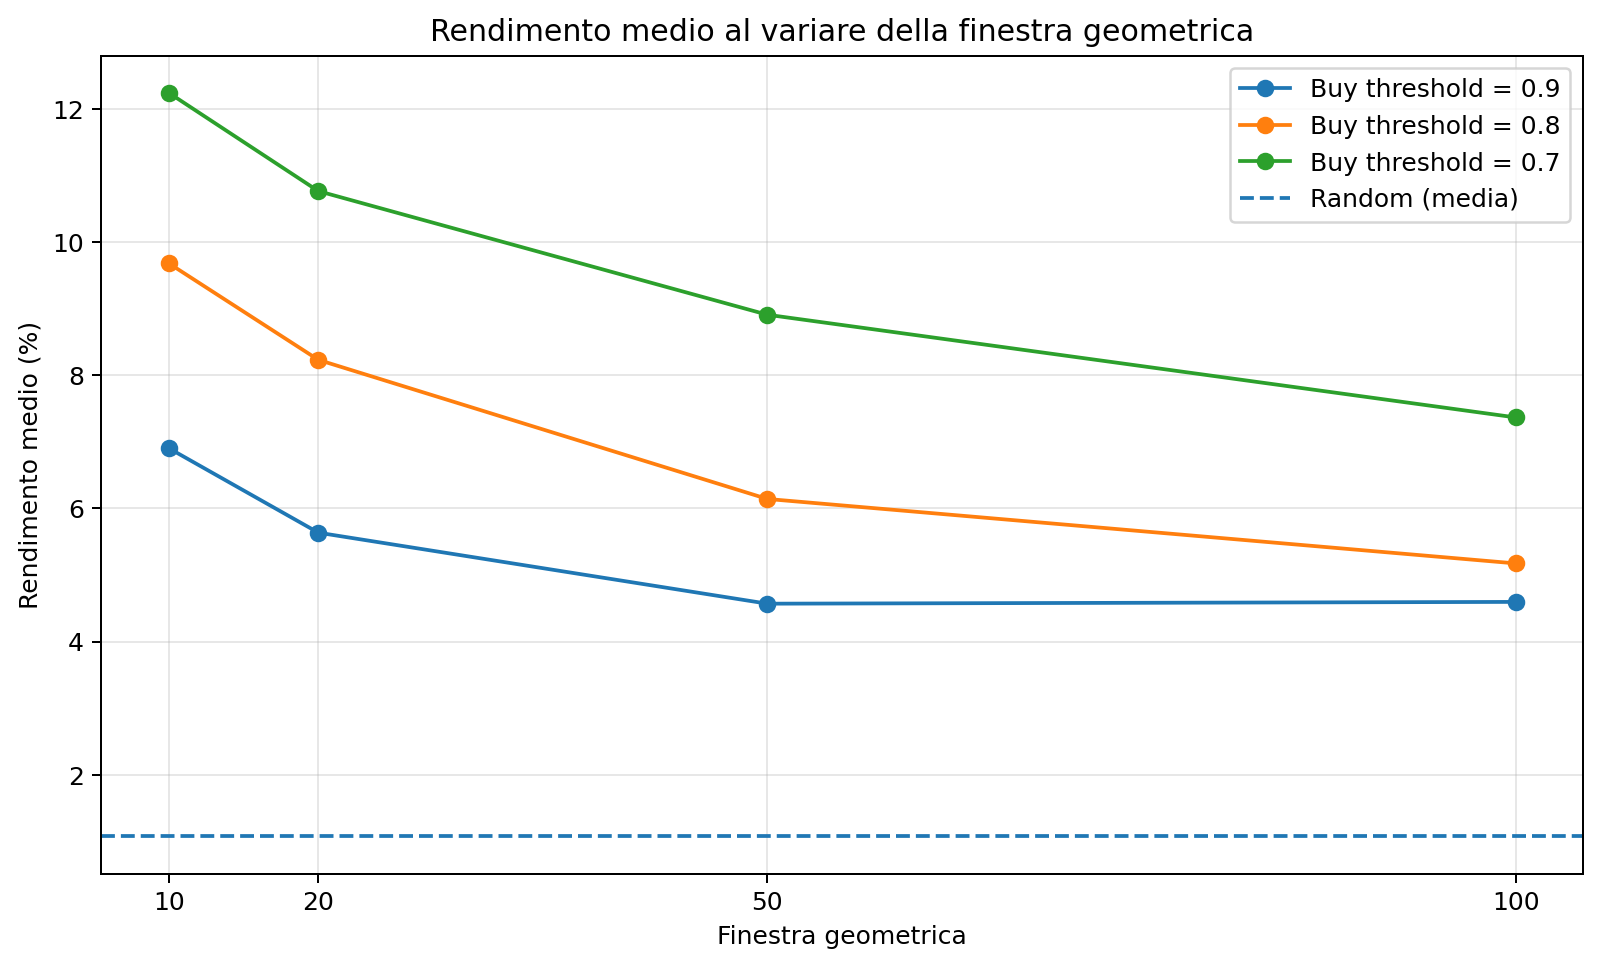
\includegraphics[width=0.95\textwidth]{grafici/01_rendimento_finestra_valori.png}%
    }{%
        \fbox{\parbox{0.85\textwidth}{\centering Grafico non disponibile}}%
    }%
}
\caption{Average Yield al variare della finestra geometrica e della soglia
di acquisto, con capitale accantonato pari al 10\%.}
\label{fig:yield_window}
\end{figure}

Come mostrato in Figura~\ref{fig:yield_window}, per tutte le soglie
considerate il rendimento tende a diminuire all'aumentare della finestra
geometrica.

L'effetto è particolarmente evidente per la soglia di acquisto pari a 0.7,
per la quale il rendimento passa dal 12.2462\% con finestra 10 al 10.7685\%
con finestra 20, all'8.91111\% con finestra 50 e infine al 7.36828\% con
finestra 100.

Per la soglia 0.8 il rendimento passa invece dal 9.6844\% con finestra 10 al
5.17482\% con finestra 100. Con soglia 0.9 si passa dal 6.90619\% al
4.59632\%.

Il grafico permette quindi di osservare contemporaneamente l'effetto della
finestra geometrica e quello della soglia di acquisto, mantenendo costante la
percentuale di capitale accantonato.

Anche la deviazione standard è stata analizzata al variare dei parametri. I
risultati sono riportati in Figura~\ref{fig:std_window}.

\begin{figure}[ht]
\centering
\IfFileExists{relazione/grafici/02_deviazione_standard_finestra_valori.png}{%
    \includegraphics[width=0.95\textwidth]{relazione/grafici/02_deviazione_standard_finestra_valori.png}%
}{%
    \IfFileExists{grafici/02_deviazione_standard_finestra_valori.png}{%
        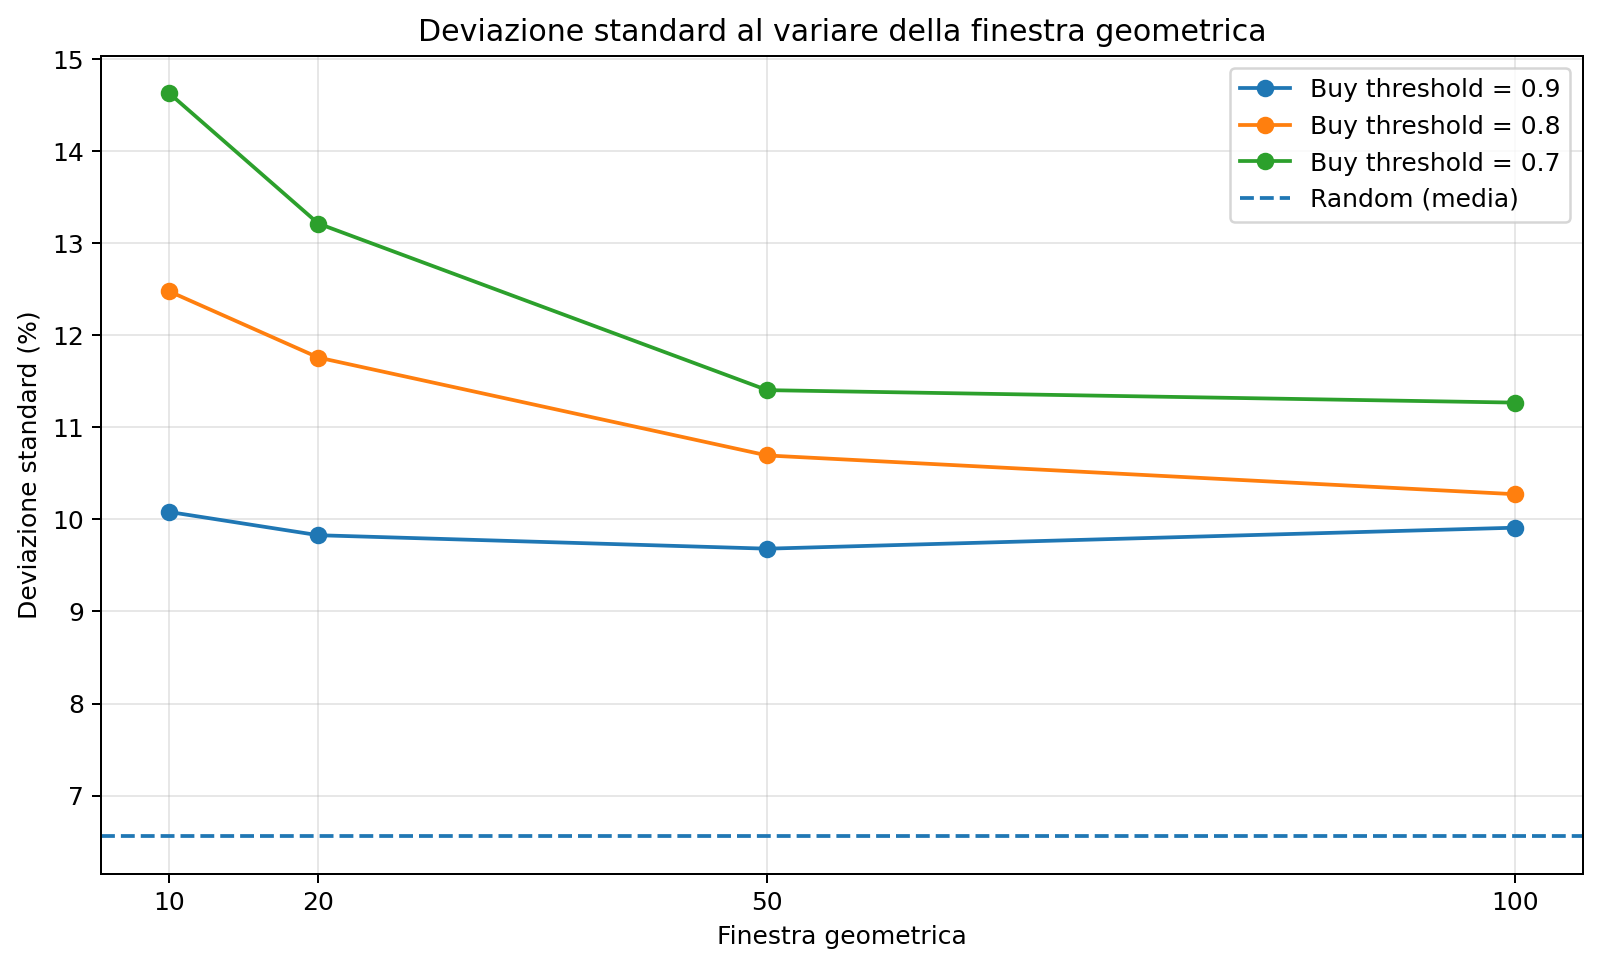
\includegraphics[width=0.95\textwidth]{grafici/02_deviazione_standard_finestra_valori.png}%
    }{%
        \fbox{\parbox{0.85\textwidth}{\centering Grafico non disponibile}}%
    }%
}
\caption{Deviazione standard al variare della finestra geometrica e della
soglia di acquisto, con capitale accantonato pari al 10\%.}
\label{fig:std_window}
\end{figure}

Per la soglia 0.7, la deviazione standard diminuisce da 14.6348\% con
finestra 10 a 13.214\% con finestra 20, fino a 11.269\% con finestra 100.
Anche per la soglia 0.8 si osserva una diminuzione, da 12.48\% con finestra
10 a 10.2738\% con finestra 100.

Per la soglia 0.9 la variazione è invece più contenuta: la deviazione standard
passa dal 10.0821\% con finestra 10 al 9.82848\% con finestra 20 e al
9.68225\% con finestra 50, per poi aumentare leggermente fino al 9.91048\%
con finestra 100.

I risultati mostrano quindi che il cambiamento della finestra geometrica
influenza sia il rendimento medio sia la variabilità dei risultati.

Un'ulteriore analisi riguarda direttamente la soglia di acquisto. La
Figura~\ref{fig:yield_threshold} mostra il rendimento medio per le diverse
finestre geometriche.

\begin{figure}[ht]
\centering
\IfFileExists{relazione/grafici/03_rendimento_soglia_valori.png}{%
    \includegraphics[width=0.95\textwidth]{relazione/grafici/03_rendimento_soglia_valori.png}%
}{%
    \IfFileExists{grafici/03_rendimento_soglia_valori.png}{%
        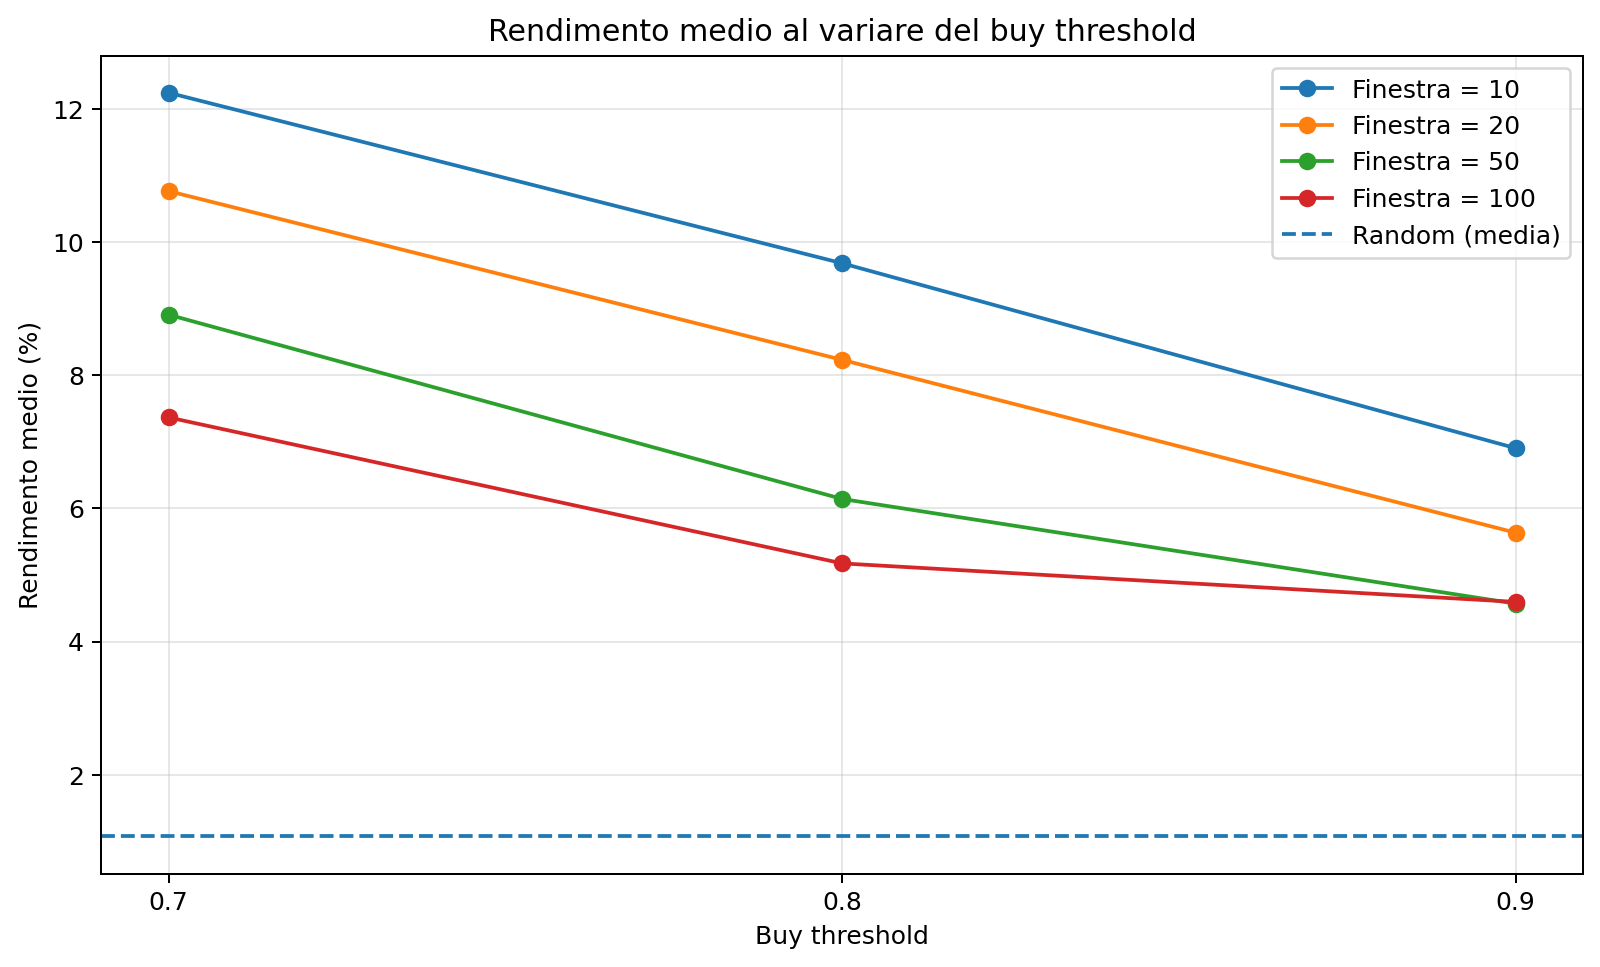
\includegraphics[width=0.95\textwidth]{grafici/03_rendimento_soglia_valori.png}%
    }{%
        \fbox{\parbox{0.85\textwidth}{\centering Grafico non disponibile}}%
    }%
}
\caption{Average Yield al variare della soglia di acquisto per le diverse
finestre geometriche, con capitale accantonato pari al 10\%.}
\label{fig:yield_threshold}
\end{figure}

La Figura~\ref{fig:yield_threshold} mostra che, per tutte le finestre
considerate, la riduzione della soglia di acquisto da 0.9 a 0.7 è associata
a un aumento del rendimento medio.

È importante osservare che una soglia più bassa non rappresenta una maggiore
permissività della strategia. Nel caso considerato, l'acquisto viene
effettuato quando il rapporto tra il prezzo corrente e la media geometrica è
inferiore alla soglia. Di conseguenza, una soglia pari a 0.7 richiede un
rapporto più basso rispetto a una soglia pari a 0.9.

\subsection{Influenza del capitale accantonato}

È stato analizzato anche l'effetto della percentuale di capitale accantonata.
Nella maggior parte delle configurazioni della strategia Smart, il valore
del rendimento rimane invariato al variare di questo parametro.

Ad esempio, per una finestra geometrica pari a 10 e una soglia di acquisto
pari a 0.7, il rendimento medio è pari a 12.2462\% per tutte le percentuali
di capitale accantonato considerate.

\begin{table}[ht]
\centering
\caption{Average Yield al variare del capitale accantonato con finestra
geometrica pari a 10.}
\label{tab:setaside_window10}
\begin{tabularx}{\textwidth}{>{\centering\arraybackslash}X|>{\centering\arraybackslash}X|>{\centering\arraybackslash}X|>{\centering\arraybackslash}X}
\hline
\textbf{Set Aside (\%)} &
\textbf{Buy 0.9} &
\textbf{Buy 0.8} &
\textbf{Buy 0.7} \\
\hline
10 & 6.90619 & 9.68440 & 12.2462 \\
20 & 6.90593 & 9.68440 & 12.2462 \\
30 & 7.14284 & 9.68440 & 12.2462 \\
50 & 7.51935 & 9.77596 & 12.2462 \\
\hline
\end{tabularx}
\end{table}

La Tabella~\ref{tab:setaside_window10} mostra che l'effetto del capitale
accantonato dipende dalla configurazione utilizzata. Per le soglie 0.8 e
0.7 le variazioni sono molto contenute, mentre con soglia 0.9 si osserva un
aumento del rendimento passando dal 6.90619\% al 7.51935\%.

Il comportamento è mostrato anche nella Figura~\ref{fig:setaside_yield}.

\begin{figure}[ht]
\centering
\IfFileExists{relazione/grafici/04_rendimento_set_aside_valori.png}{%
    \includegraphics[width=0.95\textwidth]{relazione/grafici/04_rendimento_set_aside_valori.png}%
}{%
    \IfFileExists{grafici/04_rendimento_set_aside_valori.png}{%
        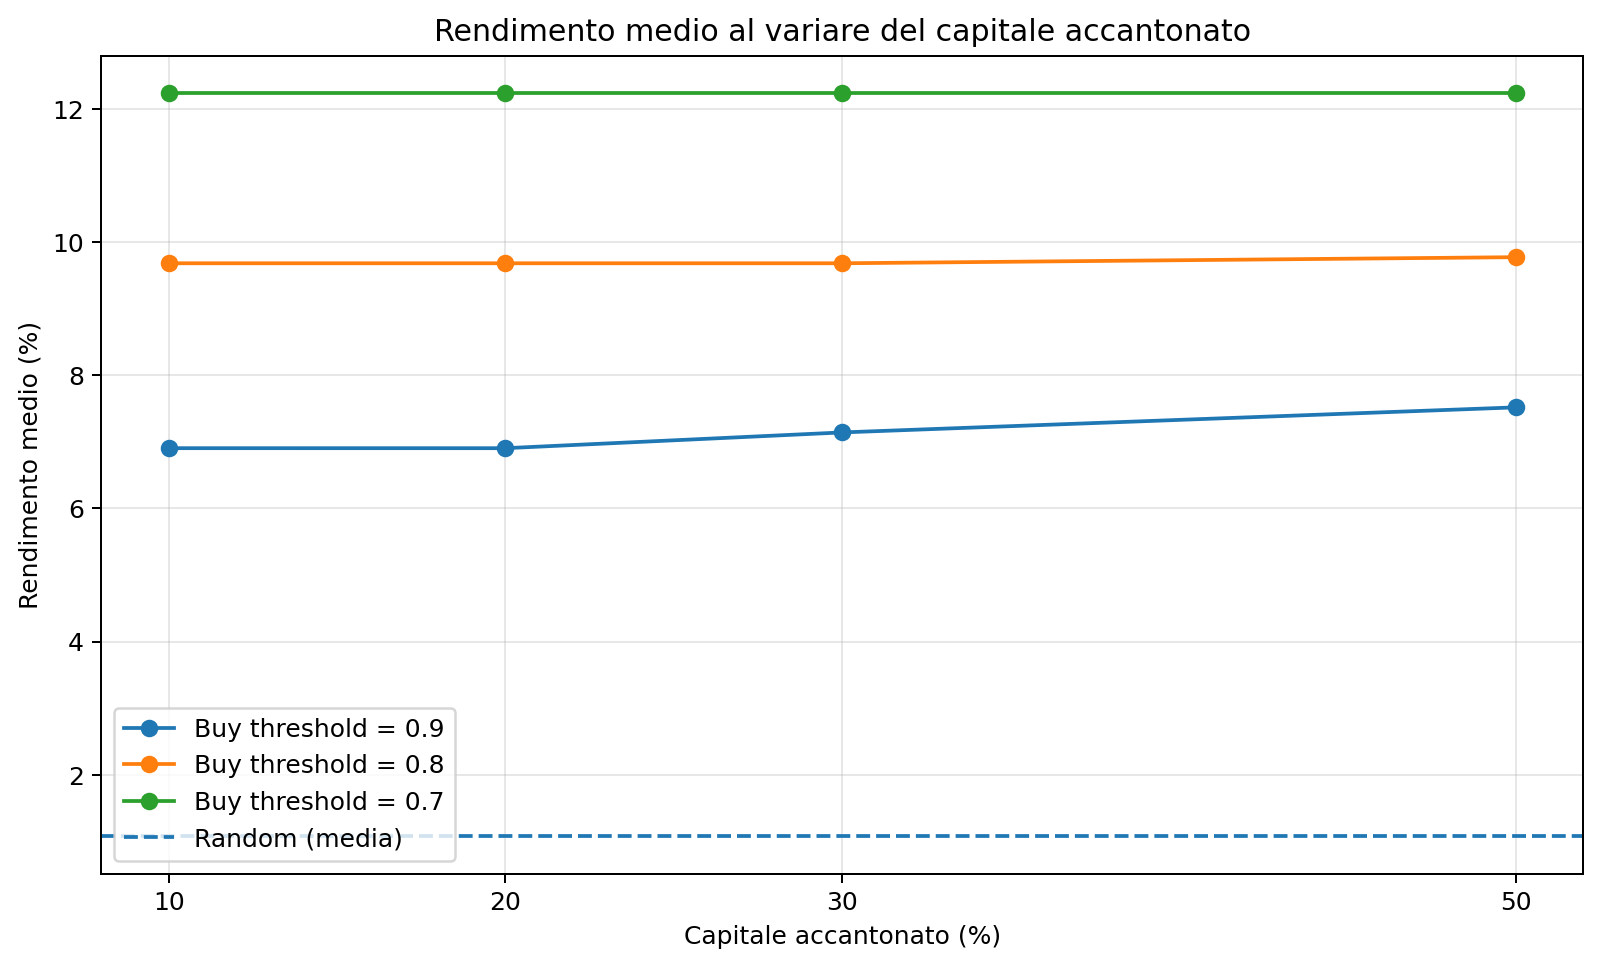
\includegraphics[width=0.95\textwidth]{grafici/04_rendimento_set_aside_valori.png}%
    }{%
        \fbox{\parbox{0.85\textwidth}{\centering Grafico non disponibile}}%
    }%
}
\caption{Average Yield al variare del capitale accantonato per le diverse
soglie di acquisto, con finestra geometrica pari a 10.}
\label{fig:setaside_yield}
\end{figure}

\subsection{Confronto con la baseline casuale}

La strategia \texttt{randomChoise} viene utilizzata come baseline per il
confronto con la strategia basata sulla media geometrica.

La baseline è stata eseguita con una finestra geometrica indicata nei
parametri pari a 20 e con soglia di acquisto pari a 0.8, ma tali parametri
non influenzano la scelta casuale effettuata dalla strategia. L'unico
parametro analizzato per la baseline è quindi la percentuale di capitale
accantonato.

I risultati ottenuti sono riportati nella Tabella~\ref{tab:random_results}.

\begin{table}[ht]
\centering
\caption{Risultati della baseline casuale al variare del capitale
accantonato.}
\label{tab:random_results}
\begin{tabularx}{\textwidth}{>{\centering\arraybackslash}X|>{\centering\arraybackslash}X|>{\centering\arraybackslash}X|>{\centering\arraybackslash}X}
\hline
\textbf{Set Aside (\%)} &
\textbf{Average Yield (\%)} &
\textbf{Deviazione standard (\%)} &
\textbf{Variazione media del saldo} \\
\hline
10 & 0.604743 & 8.57587 & 6.04743 \\
20 & 1.28263  & 7.29516 & 12.8263 \\
30 & 1.31554  & 5.97585 & 13.1554 \\
50 & 1.09330  & 4.38354 & 10.9330 \\
\hline
\end{tabularx}
\end{table}

Nel campione analizzato, il rendimento medio della baseline varia quindi da
0.604743\% a 1.31554\%. La deviazione standard varia invece da 4.38354\% a
8.57587\%.

Per confrontare in modo sintetico le due strategie è possibile considerare
gli intervalli dei valori osservati.

\begin{table}[ht]
\centering
\caption{Confronto tra gli intervalli osservati per le strategie Random
e Smart.}
\label{tab:strategy_comparison}
\begin{tabularx}{\textwidth}{>{\centering\arraybackslash}X|>{\centering\arraybackslash}X|>{\centering\arraybackslash}X|>{\centering\arraybackslash}X}
\hline
\textbf{Strategia} &
\textbf{Yield min--max (\%)} &
\textbf{Dev. standard min--max (\%)} &
\textbf{Variazione saldo min--max} \\
\hline
Random & 0.604743--1.31554 & 4.38354--8.57587 &
6.04743--13.1554 \\

Smart & 4.56965--12.2462 & 9.68035--14.6348 &
45.6965--122.462 \\
\hline
\end{tabularx}

\end{table}

Nel campione analizzato, tutte le configurazioni Smart considerate presentano
un rendimento medio superiore a quello delle configurazioni Random. Il valore
minimo osservato per Smart è infatti pari a 4.56965\%, mentre il valore
massimo osservato per Random è pari a 1.31554\%.

Anche la deviazione standard presenta valori più elevati per la strategia
Smart. Il valore minimo osservato per Smart è pari a 9.68035\%, mentre il
valore massimo osservato per Random è pari a 8.57587\%.

Il confronto deve comunque essere interpretato considerando Random come
baseline e non come una configurazione equivalente alle diverse
configurazioni Smart. La strategia casuale infatti non utilizza la finestra
geometrica e la soglia di acquisto per determinare le operazioni.

\subsection{Discussione}

I risultati mostrano una relazione tra il rendimento medio e la variabilità
delle configurazioni analizzate. In particolare, le configurazioni con
rendimento medio maggiore presentano in diversi casi anche una deviazione
standard maggiore.

Un esempio è rappresentato dalla finestra geometrica pari a 10 e dal
capitale accantonato pari al 10\%. Riducendo la soglia di acquisto da 0.9 a
0.7, il rendimento medio passa dal 6.90619\% al 12.2462\%, mentre la
deviazione standard passa dal 10.0821\% al 14.6348\%.

Anche la finestra geometrica influenza il risultato. Con soglia di acquisto
pari a 0.7 e capitale accantonato pari al 10\%, aumentando la finestra da 10
a 100 timestamp il rendimento medio diminuisce dal 12.2462\% al 7.36828\%.

Nel dataset utilizzato, quindi, le finestre più brevi sono associate a
rendimenti medi maggiori per le configurazioni considerate. Questo risultato
deve essere riferito ai dati e alle configurazioni utilizzate nell'esperimento
e non viene esteso a dataset differenti.

La percentuale di capitale accantonato presenta invece variazioni più
limitate. In particolare, per diverse combinazioni di finestra e soglia il
rendimento rimane invariato al variare di questo parametro. In altri casi si
osservano variazioni contenute, come nella configurazione con finestra 10 e
soglia 0.9, nella quale il rendimento passa dal 6.90619\% con capitale
accantonato pari al 10\% al 7.51935\% con capitale accantonato pari al 50\%.

Nel complesso, nel campione analizzato la strategia
\texttt{smartgeometricChoise} presenta rendimenti medi superiori rispetto
alla baseline casuale per tutte le configurazioni considerate. Allo stesso
tempo, presenta anche valori di deviazione standard generalmente maggiori.

Per questo motivo il solo rendimento medio non è sufficiente a descrivere il
comportamento della strategia. La deviazione standard permette infatti di
considerare anche la variabilità dei risultati e di osservare il compromesso
presente tra rendimento medio e variabilità.
\chapter{Conclusioni}

\label{chap:conclusions}

Il lavoro svolto ha portato alla realizzazione di un simulatore per lo studio
di strategie di compravendita di energia elettrica a partire da serie storiche
di prezzi. Il sistema permette di modellare le principali componenti coinvolte
nel processo di compravendita, gestire le operazioni di acquisto e vendita e
ripetere le simulazioni su diverse configurazioni.
La struttura del simulatore è stata progettata in modo da separare il caricamento
dei dati, il modello del dominio, la gestione delle operazioni di trading
e l'esecuzione delle simulazioni. Questa organizzazione permette di utilizzare
strategie differenti mantenendo invariati i principali vincoli economici ed energetici del sistema.

\section{Sintesi}

L'obiettivo principale del lavoro era verificare se l'utilizzo dello storico dei
prezzi attraverso una media geometrica potesse portare a risultati differenti rispetto
a una strategia che effettua le proprie scelte in modo casuale.
I risultati ottenuti mostrano che, nel dataset e nelle configurazioni considerate,
la strategia \texttt{smartgeometricChoise} ha prodotto rendimenti medi superiori rispetto
alla baseline casuale. Le configurazioni Smart considerate hanno infatti ottenuto rendimenti
medi compresi tra il 4.56965% e il 12.2462%, mentre quelli della baseline casuale sono
compresi tra lo 0.604743% e l'1.31554%.
Questo risultato è però accompagnato da una maggiore variabilità. La deviazione standard
osservata per la strategia Smart è infatti superiore a quella osservata per la baseline
casuale nel campione analizzato. Questo mostra che un rendimento medio maggiore non è
sufficiente, da solo, per descrivere il comportamento di una strategia, ma deve essere
considerato insieme alla variabilità dei risultati.
Gli esperimenti hanno inoltre mostrato un'influenza dei parametri utilizzati dalla strategia.
In particolare, nel dataset considerato, le configurazioni con finestre geometriche più brevi
hanno generalmente prodotto rendimenti medi maggiori. Anche la soglia di acquisto ha avuto un
effetto rilevante: riducendo la soglia da 0.9 a 0.7, il rendimento medio è aumentato nelle
configurazioni analizzate, insieme alla deviazione standard.
Il parametro relativo al capitale accantonato ha invece mostrato un'influenza più limitata.
In diverse configurazioni il rendimento è rimasto invariato, mentre in altre si sono osservate variazioni contenute.
I risultati ottenuti devono comunque essere riferiti alle serie storiche e alle configurazioni
utilizzate nell'esperimento. Non è quindi possibile considerare la strategia Smart come
generalmente migliore della baseline sulla base dei soli esperimenti effettuati. Il lavoro
mostra piuttosto che l'utilizzo della media geometrica può produrre risultati differenti dalla
scelta casuale e che tali risultati dipendono dai parametri utilizzati e dai dati sui quali
viene eseguita la simulazione.

\section{Sviluppi futuri}

Il simulatore realizzato può essere ulteriormente esteso sia dal punto di vista delle
strategie sia da quello della valutazione sperimentale.
Un primo possibile sviluppo consiste nell'introduzione di ulteriori strategie di trading
e di altri indicatori statistici, in modo da poter confrontare approcci differenti
utilizzando lo stesso ambiente di simulazione.
Un secondo sviluppo riguarda l'utilizzo di dataset più ampi e diversificati. L'analisi
potrebbe essere ripetuta su serie storiche provenienti da periodi differenti o da mercati
differenti, verificando se i risultati osservati rimangono simili anche in condizioni diverse.
Un ulteriore aspetto riguarda la scelta dei parametri. Nel lavoro i parametri delle strategie
vengono variati nelle diverse configurazioni sperimentali. In futuro potrebbe essere introdotta
una procedura automatica per la loro selezione. Tale procedura dovrebbe però separare i dati
utilizzati per la scelta dei parametri da quelli utilizzati per la valutazione finale, in modo
da evitare di selezionare una configurazione sulla base degli stessi dati sui quali viene poi
misurato il risultato.
Dal punto di vista dell'implementazione, sarebbe inoltre possibile approfondire la valutazione
delle prestazioni del simulatore, raccogliendo in modo sistematico i tempi di esecuzione e
l'utilizzo della memoria al variare del numero di thread utilizzati. Questo permetterebbe di valutare
più precisamente l'effetto della parallelizzazione introdotta tramite OpenMP.
Infine, il sistema potrebbe essere arricchito con un insieme più ampio di test automatici sulle
principali invarianti del modello, in particolare per la batteria, il portafoglio e il servizio
di trading. Questo permetterebbe di verificare automaticamente il rispetto dei vincoli del sistema
anche in seguito all'introduzione di nuove funzionalità o strategie.

\backmatter
\cleardoublepage
\phantomsection
\addcontentsline{toc}{chapter}{\bibname}
\bibliographystyle{plain}
\bibliography{references}

\end{document}
